%%%%%%%%%%%%%%%%%%%%%%%%%%%%%%%%%%%%%%%%%%%%%%%%%%%%%%%%%%%%%%%%%%%
% 
% $Id: sec5.tex,v 1.1.1.1 2002/01/02 19:36:28 phil Exp $
%
% $Log: sec5.tex,v $
% Revision 1.1.1.1  2002/01/02 19:36:28  phil
% initial import into CVS
%
% Revision 1.10  1997/08/29 20:06:11  allen
% *** empty log message ***
%
% Revision 1.9  1997/08/28 16:38:38  cguo
% *** empty log message ***
%
% Revision 1.8  1996/08/13 17:11:09  cguo
% *** empty log message ***
%
% Revision 1.7  1996/08/13 00:56:12  cguo
% glossary a problem
%
% Revision 1.6  1996/08/12 23:25:17  cguo
% ready for phil
%
% Revision 1.5  1996/08/06 21:39:49  cguo
% *** empty log message ***
%
% Revision 1.4  1996/08/02 22:18:16  cguo
% *** empty log message ***
%
% Revision 1.3  1996/04/29 19:03:29  stockie
% ready for carmen
%
% Revision 1.2  1995/08/14  22:20:25  stockie
% - add glossary terms
% - change labels to depend on lab #
% - use new versions of \quiz, \demo, \technicalnote, etc.
% - add comments to figures
% - define saturation ratio
% - add other approximations for first derivative
% - change summary
%
% Revision 1.1  1995/07/18  21:39:08  stockie
% Initial revision
%
%
%%%%%%%%%%%%%%%%%%%%%%%%%%%%%%%%%%%%%%%%%%%%%%%%%%%%%%%%%%%%%%%%%%%

\section{Difference Approximations to the First Derivative}
\label{lab1:sec:diff-first-deriv}

%%%%%%%%%%%%%%%%%%%
\begin{latexonly}
\gloss{finite difference}{an approximation of the derivative of a
  function by a
  difference quotient involving values of the function at discrete
  points.  The simplest method of deriving finite difference formulae
  is using Taylor series.}
\gloss{backward difference discretization}{used to estimate a derivative
-- uses the current points and points with smaller independent variable.}
\gloss{centre difference discretization}{used to estimate a derivative
-- uses a discretization symmetric (in independent variable) around the
current point.}
\gloss{converge}{as the discretization step (eg. $\Delta t$) is reduced
the solutions generated approach one solution curve.}
\gloss{numerical instability}{although the continuous differential equation
has a finite solution, the numerical solution grows without bound as the 
numerical interation proceeds.}
\end{latexonly}
%%%%%%%%%%%%%%%%%%%
It only remains to write a discrete version of the
differential equation \eqref{lab1:eq:conduction} involving the approximations 
$T_i$.    
The way we do this is to approximate the derivatives with 
\emph{finite differences}.  
\index{finite difference}
If this term is new to you, then you can think of it
as just another name for a concept you have already seen in calculus.
Remember the \emph{definition of the derivative of a function $y(t)$},
where $y^\prime(t)$ is 
written as a limit of a divided difference:
\begin{equation}
  y^\prime(t) = \lim_{\dt\rightarrow 0} \frac{y(t+\dt)-y(t)}{\dt}.
  \label{lab1:eq:defn-deriv}
\end{equation}
We can apply the same idea to approximate the derivative
$dT/dt=T^\prime$ in  
\eqref{lab1:eq:conduction} by the \emph{forward difference formula}, using
the discrete approximations, $T_i$:
\index{forward difference formula}
\begin{equation}
  T^\prime(t_i) \approx \frac{T_{i+1}-T_i}{\dt}.
  \label{lab1:eq:forward-diff}
\end{equation}

\begin{example}
\begin{latexonly}
  In order to understand the ability of the formula
  \eqref{lab1:eq:forward-diff} to approximate the derivative, 
  let's look at a specific example.
  Take the function $y(x)=x^3-5x$, and apply the forward difference
  formula at the point $x=1$.  The function and its tangent line (the
  short line segment with slope $y^\prime(1)$) are displayed in
  Figure~\ref{lab1:fig:deriv}.
  
  Each of the remaining line segments represents the forward
  difference approximation to the tangent line for different values of
  \dt, which are simply \emph{the secant lines through the points
    $(t,y(t))$ and $(t+\dt,y(t+\dt))$}.
  Notice that the approximation improves as \dt\ is reduced.
  This motivates the idea that grid refinement improves the accuracy
  of the discretization \dots but not always (as we will see in
  the coming sections).
  \begin{figure}[htbp]
    \begin{center}
      \leavevmode
%%%%%%%%%%%%%%%%%%%%%%%%%%%%%%%%%%%%%%%%%%%%%%%%%%%%%
%  NOTE: This plot is produced by the Gnuplot script
%  ``deriv/deriv.gin''.
%%%%%%%%%%%%%%%%%%%%%%%%%%%%%%%%%%%%%%%%%%%%%%%%%%%%%
      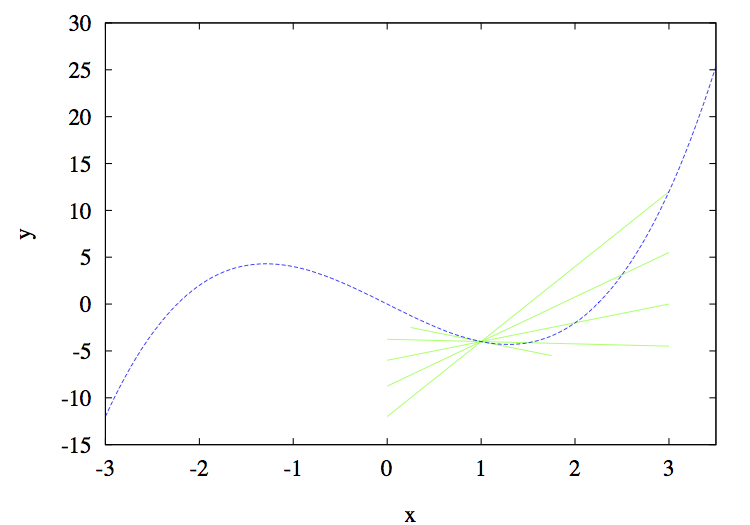
\includegraphics[height=3.5in]{deriv/deriv}      
      \caption{Plot of the function $y=x^3-5x$ and the forward difference approximations to the derivative for various values of \dt.}
      \label{lab1:fig:deriv}
    \end{center}
  \end{figure}
\end{latexonly}

\demo{deriv.cgi}{Investigate the use of the forward difference
  formula to approximate derivatives here.\label{lab1:demo:deriv}}

%\technicalnote{Details on how the derivative example works\dots}{See Appendix }{ for details on how the derivative example works.}{lab1:tech:deriv} 

\end{example}

%%%%%%%%%%%%%%%%%%%%%%%%%%%%%%%%%%%%%%%%%%%%%%%%%%%%%%%%%%%%%%%%%%%%%%%
\subsection{Forward Euler Method}
\label{lab1:sec:forward-euler}

We can now write down a discrete version of our model ODE problem
\eqref{lab1:eq:conduction} at any point \ti\ by
\begin{enumerate}
\item discretizing the derivative on the left hand side (for example,
  using the forward difference approximation~\eqref{lab1:eq:forward-diff});
\item evaluating the right hand side function at the discrete point
  \ti.
\end{enumerate}
The discrete form of the problem is 
\[
  \frac{T_{i+1}-T_i}{\dt} = \lambda(T_i,t_i) \, (T_i-T_a),
\]
or, after rearranging,
\begin{equation}
  T_{i+1} = T_i + \dt \, \lambda(T_i,t_i) \, (T_i-T_a).
  \label{lab1:eq:forward-euler-conduction}
\end{equation}
This formula is called the \emph{Forward Euler method}
\index{forward Euler method}
(since it uses forward differences).
Notice that this formula relates each discrete solution value to the
solution at the preceding $t$-point.
Consequently, if we are given an initial value $T(0)$, then all
subsequent values of the solution are easily computed.  

({\bf Note:} The forward Euler formula for the more general
first-order IVP in~\eqref{lab1:eq:modelode} is simply 
$y_{i+1} = y_i + \dt f(y_i,t_i)$.)

\begin{example}
  \label{lab1:exm:saturation}
  Let us now turn to another example in atmospheric physics to
  illustrate the use of the forward Euler method. 
  Consider the process of condensation and evaporation in a cloud. 
  The \emph{saturation ratio}, $S$, is the ratio of the vapour pressure
  to the vapour pressure of a plane surface of water at temperature
  $T$.  $S$ varies in time according to the saturation development
  equation 
  \begin{equation}
    \frac{dS}{dt} = \alpha S^2 + \beta S + \gamma,
    \label{lab1:eq:saturation}
  \end{equation}
  where $\alpha$, $\beta$ and $\gamma$ are complicated (but constant)
  expressions involving the physical parameters in the problem (and so
  we won't reproduce them here).  

  \begin{note}
    What are some physically reasonable values of the
    parameters (other than simply $\alpha<0$ and $\gamma>0$)?   
  \end{note}

  ~\cite{chen} gives a detailed derivation of the equation, which
  is a non-linear, first order ODE (\ie~non-linear in the dependent
  variable $S$, and it contains only a
  first derivative in the time variable). 
  Chen also derives an analytical solution to the problem which takes
  a couple pages of messy algebra to come to.
  Rather than show these
  details, we would like to use the forward Euler method in order to
  compute the solution numerically, and as we will see, this is
  actually quite simple.

  Using the forward difference formula \eqref{lab1:eq:forward-diff}, the
  discrete form of~\eqref{lab1:eq:saturation} is 
  \[
  S_{i+1} = S_i + \Delta t \left( \alpha S_i^2 + \beta S_i +
    \gamma \right).
  \]
  Consider an initial saturation ratio of $0.98$, and take parameter
  values $\alpha=-1$, $\beta=1$ and $\gamma=1$.  
%%%%%%%%%%%%%%%%%
  The resulting solution, for various values of the time step \dt,is
  plotted in Figure~\ref{lab1:fig:saturation}. 
  \begin{figure}[htbp]
    \begin{center}
      \leavevmode
%%%%%%%%%%%%%%%%%%%%%%%%%%%%%%%%%%%%%%%%%%%%%%%%%%%%%
%  NOTE: This plot is produced by the Gnuplot script
%  ``feuler/fe.gin'' and the data files 
%  ``feuler/fe*.out'' (the data were obtained using
%  the simple C program ``feuler/fe.c'', executable file  
%  ``feuler/fe'').  
%%%%%%%%%%%%%%%%%%%%%%%%%%%%%%%%%%%%%%%%%%%%%%%%%%%%%
      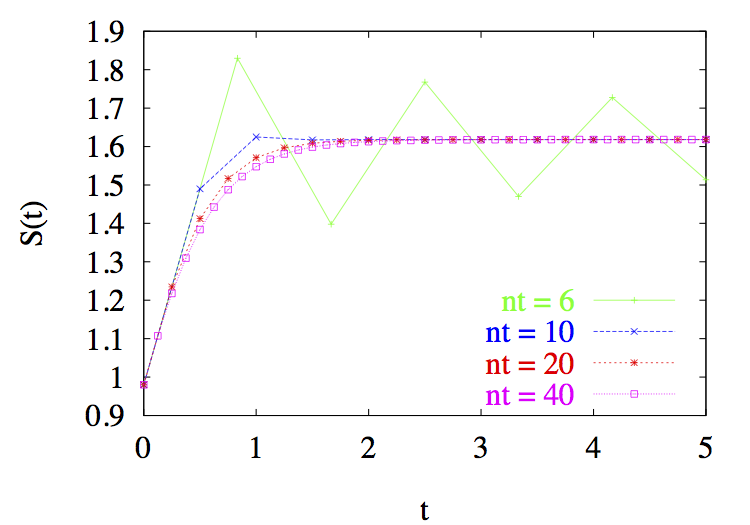
\includegraphics[height=3.5in]{feuler/sat2}      
      \caption{Plot of the saturation ratio as a function of time
        using the Forward Euler method. ``{\tt{nt}}'' is the number of
        time steps.}
      \label{lab1:fig:saturation}
    \end{center}
  \end{figure}

%\demo{saturation.cgi}{Here is an interactive demonstration of the
%  solution to the saturation problem \dots NOT AVAILABLE YET!!!
%  \label{lab1:demo:saturation}} 
%
%%%%%%%%%%%%

  There are two things to notice here, both related to the importance of
  the choice of time step \dt\ :
  \begin{itemize}
  \item As \dt\ is reduced, the solution appears to \emph{converge}
    to one solution curve, which we would hope is the exact solution
    to the differential equation.  An important question to ask is:
    \emph{When will the numerical method converge to the exact
      solution as \dt\ is reduced?}   
  \item If \dt\ is taken too large, however, the numerical solution
    breaks down.  In the above example, the oscillations that occur
    for the largest time step (when $nt=6$) are a sign of {\em
      numerical instability}.  The differential problem is stable
    and exhibits no such behaviour, but the numerical scheme we have
    used has introduced an instability.
    An obvious question that arises is: \emph{How can we avoid
      introducing instabilities in a numerical scheme?}
  \end{itemize}
  Neither question has an obvious answer, and both issues will be
  investigated further in \htmladdnormallink{Lab~\#2}{\LabtwoURL}
\end{example}

%%%%%%%%%%%%%%%%%%%%%%%%%%%%%%%%%%%%%%%%%%%%%%%%%%%%%%%%%%%%%%%%%%%%%%%
\subsection{Other Approximations}

Look again at the limit definition of
derivative~\eqref{lab1:eq:defn-deriv}, and notice that an equivalent
expression for $T^\prime$ is 
\begin{equation}
  T^\prime(t) = \lim_{\dt\rightarrow 0} \frac{T(t)-T(t-\dt)}{\dt}.
  \label{lab1:eq:defn-back}
\end{equation}
From this, we can derive the \emph{backward difference formula} for the
first derivative, 
\begin{equation}
  T^\prime(t_i) \approx \frac{T_i-T_{i-1}}{\dt},
  \label{lab1:eq:backward-diff}
\end{equation}
and similarly the \emph{centered difference formula}
\begin{equation}
  T^\prime(t_i) \approx \frac{T_{i+1}-T_{i-1}}{2 \dt}.
  \label{lab1:eq:centered-diff}
\end{equation}

The corresponding limit formulas are equivalent from a mathematical
standpoint, {\bf but the discrete formulas are not!}  
In particular, the accuracy and stability of numerical schemes derived
from the three difference formulas \eqref{lab1:eq:forward-diff},
\eqref{lab1:eq:backward-diff} and \eqref{lab1:eq:centered-diff} are
quite different.
More will be said on this in the next
Lab~\externalref{lab2secfirstderiv}. 

%%%%%%%%%%%%%%%%%%%%%%%%%%%%%%%%%%%%%%%%%%%%%%%%%%%%%%%%%%%%%%%%%%%%%%%
\paragraph{Summary}

This section introduces the use of the forward difference formula to
discretize the derivatives in a first order differential equation.
The resulting numerical scheme is called the forward Euler method.  
We also introduced the backward and centered difference formulas for
the first derivative, which were also obtained from the definition of 
derivative.  

You saw how the choice of grid spacing affected the accuracy of the
solution, and were introduced to the concepts of convergence and
stability of a numerical scheme.
More will be said about these topics in the succeeding lab,
as well as other methods for discretizing derivatives.

%%% Local Variables: 
%%% mode: latex
%%% TeX-master: "lab1"
%%% End: 
